\clearpage

\section{Descartes ja kaksinkertainen kulma}

Piru Descartes löytää yöllisen retkensä aikana maahan piirretyn terävän kulman. Descartes kärsii ahdistuneisuushäiriöistä eikä kulma mielytä häntä. Hän haluaisi että kulma on tasan kaksinkertainen alkuperäiseen nähden. Hänellä on kuitenkin mukanaan ainoastaan suora keppi, harppi ja punainen liitu. Kuinka Descartes saa muutettua kulman haluamallaan tavalla?

\begin{figure}[h]
    \centering
    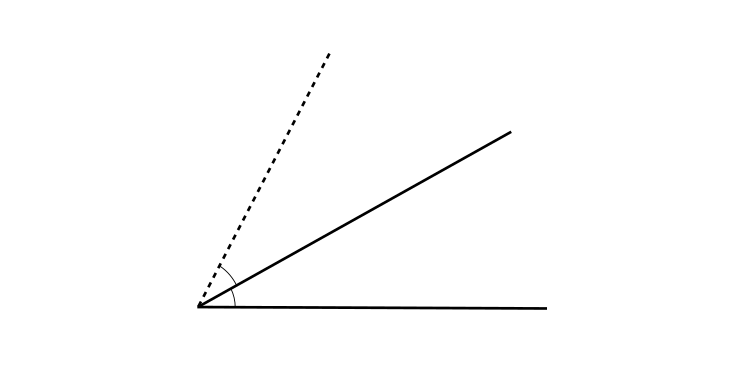
\includegraphics[width=0.7\linewidth]{kuvat/uusi_kulma.png}
\end{figure}